\documentclass[showframe,11pt]{report}\usepackage[]{graphicx}\usepackage{xcolor}
%% maxwidth is the original width if it is less than linewidth
%% otherwise use linewidth (to make sure the graphics do not exceed the margin)
\makeatletter
\def\maxwidth{ %
  \ifdim\Gin@nat@width>\linewidth
    \linewidth
  \else
    \Gin@nat@width
  \fi
}
\makeatother

\definecolor{fgcolor}{rgb}{0.196, 0.196, 0.196}
\newcommand{\hlnum}[1]{\textcolor[rgb]{0.063,0.58,0.627}{#1}}%
\newcommand{\hlstr}[1]{\textcolor[rgb]{0.063,0.58,0.627}{#1}}%
\newcommand{\hlcom}[1]{\textcolor[rgb]{0.588,0.588,0.588}{#1}}%
\newcommand{\hlopt}[1]{\textcolor[rgb]{0.196,0.196,0.196}{#1}}%
\newcommand{\hlstd}[1]{\textcolor[rgb]{0.196,0.196,0.196}{#1}}%
\newcommand{\hlkwa}[1]{\textcolor[rgb]{0.231,0.416,0.784}{#1}}%
\newcommand{\hlkwb}[1]{\textcolor[rgb]{0.627,0,0.314}{#1}}%
\newcommand{\hlkwc}[1]{\textcolor[rgb]{0,0.631,0.314}{#1}}%
\newcommand{\hlkwd}[1]{\textcolor[rgb]{0.78,0.227,0.412}{#1}}%
\let\hlipl\hlkwb

\usepackage{framed}
\makeatletter
\newenvironment{kframe}{%
 \def\at@end@of@kframe{}%
 \ifinner\ifhmode%
  \def\at@end@of@kframe{\end{minipage}}%
  \begin{minipage}{\columnwidth}%
 \fi\fi%
 \def\FrameCommand##1{\hskip\@totalleftmargin \hskip-\fboxsep
 \colorbox{shadecolor}{##1}\hskip-\fboxsep
     % There is no \\@totalrightmargin, so:
     \hskip-\linewidth \hskip-\@totalleftmargin \hskip\columnwidth}%
 \MakeFramed {\advance\hsize-\width
   \@totalleftmargin\z@ \linewidth\hsize
   \@setminipage}}%
 {\par\unskip\endMakeFramed%
 \at@end@of@kframe}
\makeatother

\definecolor{shadecolor}{rgb}{.97, .97, .97}
\definecolor{messagecolor}{rgb}{0, 0, 0}
\definecolor{warningcolor}{rgb}{1, 0, 1}
\definecolor{errorcolor}{rgb}{1, 0, 0}
\newenvironment{knitrout}{}{} % an empty environment to be redefined in TeX

\usepackage{alltt}
\usepackage{standalone}
\standalonetrue
\ifstandalone
  \usepackage{../../haziq_thesis}
  \usepackage{../../haziq_maths}
  \usepackage{../../haziq_glossary}
  \addbibresource{../../bib/haziq.bib}
  \externaldocument{../01/.texpadtmp/introduction}
  \externaldocument{../02/.texpadtmp/chapter2}
  \externaldocument{../03/.texpadtmp/chapter3}
  \externaldocument{../04/.texpadtmp/chapter4}
  \externaldocument{../05/.texpadtmp/chapter5}
  \externaldocument{../appendix/.texpadtmp/appendix}
\fi




\IfFileExists{upquote.sty}{\usepackage{upquote}}{}
\begin{document}

We present analyses of real-data examples using the I-probit model for a variety of applicaitons, namely binary and multiclass classification, meta-analysis, and spatio-temporal modelling of point processes.
Examples in this section have been analysed using in \proglang{R} using the in-development \pkg{iprobit} package written by us.
Code for replication is provided at \url{http://myphdcode.haziqj.ml}.
All of these examples had assumed a fixed error precision $\bPsi = \bI_m$.

\subsection{Predicting cardiac arrhythmia}
\index{classification!binary}
\index{cardiac arrhythmia data set}
\index{canonical kernel/RKHS}
\index{fBm kernel/RKHS}
\index{SE kernel/RKHS}

Statistical learning tools are being used in the field of medicine as a means to aid medical diagnosis of diseases.
In this example, factors determining the presence or absence of heart diseses are studied.
Traditionally, cardiologists inspect patients' cardiac activity (ECG data) in order to reach a diagnosis, which remains the ``gold standard'' method of obtaining diagnoses.
The study by \citet{guvenir1997supervised} aimed to predict cardiac abnormalities by way of machine learning, and minimise the difference between the gold standard and computer-based classifications.

The data set\footnote{Data is made publicly available at \url{https://archive.ics.uci.edu/ml/datasets/arrhythmia}.} at hand contains a myriad of ECG readings and other patient attributes such as age, height, and weight.
Altogether, there are $n=451$ observations and $p=279$ predictors.
In order for a valid comparison to be made to other studies, we excluded nominal covariates, leaving us with $p=194$ continuous predictors, which we then standardised.
In the original data set, there are 13 distinct classes of cardiac arrhythmia---again, following the lead of other studies, we had combined all forms of cardiac diseases to form a single class, thus reducing the problem to a binary classification task (normal vs. arrhythmia).

Following \cref{eq:iprobitbin}, the relationship between patient $i$'s probability of having a form of cardiac arrhthmia $p_i$ and the predictors $x_i\in\cX \equiv \bbR^{194}$ is modelled as
\begin{gather*}
  \Phi(p_i) = \alpha + f(x_i).
\end{gather*}
Further, assuming $f\in\cF$ a suitable RKHS with kernel $h_\lambda$, we may assign an I-prior on the (latent) regression function $f$.
We consider three RKHSs: the canonical (linear) RKHS, the fBm-0.5 RKHS and the SE RKHS.
The first of these three assumes an underlying linear relationship of the covariates and the probabilities, while the other two assumes a smooth relationship.
As all covariates had been standardised, it is sufficient to assign a single scale parameter $\lambda$ for the I-probit model.

For reference, fitting an I-probit model on the full data set takes about 4 seconds only, with convergence reached in at most 15 iterations.
\cref{fig:cardiac.mod.full.plot} plots the variational lower bound value over time and iterations for the cardiac arrhythmia data set.
As expected, the lower bound value increases over time until a convergence criterion is reached.




\begin{knitrout}
\definecolor{shadecolor}{rgb}{1, 1, 1}\color{fgcolor}\begin{figure}[htb]

{\centering 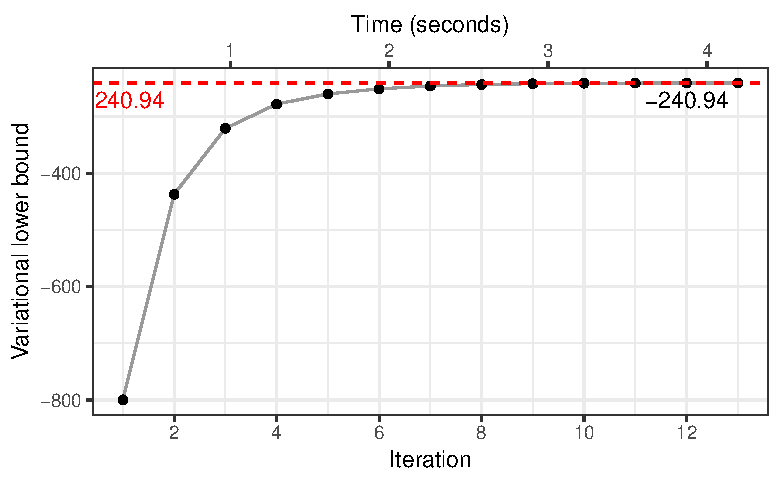
\includegraphics[width=0.785\linewidth]{figure/05-cardiac_mod_full_plot-1} 
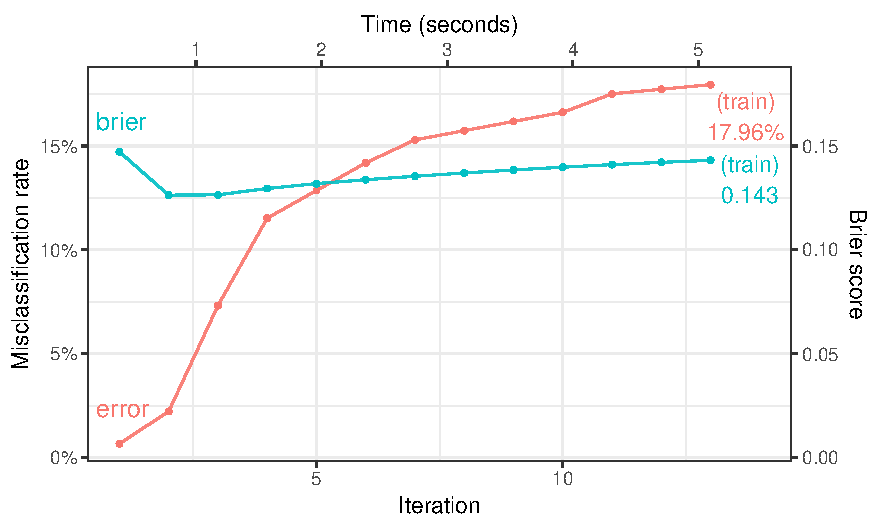
\includegraphics[width=0.785\linewidth]{figure/05-cardiac_mod_full_plot-2} 

}

\caption[Plot of variational lower bound over time (top), and plot of training error rate and Brier scores over time (bottom)]{Plot of variational lower bound over time (top), and plot of training error rate and Brier scores over time (bottom).}\label{fig:cardiac.mod.full.plot}
\end{figure}


\end{knitrout}

\index{Gaussian process!classification}
\index{linear discriminant analysis}
\index{quadratic discriminant analysis}
\index{k-nearest neighbours@$k$-nearest neighbours}
\index{support vector machine}
\index{Lasso}
To measure predictive ability, we fit the I-probit models on a random subset of the data and obtain the out-of-sample test error rates from the remaining held-out observations.
We then compare the results against popular machine learning classifiers, namely: 1) linear and quadratic discriminant analysis (LDA/QDA); 2) $k$-nearest neighbours; 3) support vector machines (SVM) \citep{steinwart2008support}; 4) Gaussian process classification \citep{rasmussen2006gaussian}; 5) random forests \citep{breiman2001random}; 6) nearest shrunken centroids (NSC) \citep{tibshirani2002diagnosis}; and 7) L-1 penalised logistic regression \citep{friedman2001elements}.
The experiment is set up as follows:
\begin{enumerate}
  \item Form a training set by sub-sampling $s \in \{50, 100, 200\}$ observations.
  \item The remaining unsampled data is used as the test set.
  \item Fit model on training set, and obtain test error rates defined as
  \[
    \text{test error rate} = \frac{1}{s} \sum_{i=1}^n [y^{\text{pred}}_i \neq y^{\text{test}}_i] \times 100 \%.
  \]
  \item Repeat steps 1-3 100 times to obtain the \emph{average} test error rates and standard errors.
\end{enumerate}
Results for the methods listed above were extracted from the in-depth study by \citet{cannings2017random}, who also conducted identical experiments using their random projection (RP) ensemble classification method.
These are all tabulated in \cref{tab:cardiac}.

\begin{table}[htb]
  \caption[Mean out-of-samle misclassification rates for the cardiac arrhythmia data set]{Mean out-of-sample misclassification rates and standard errors in parantheses for 100 runs of various training ($s$) and test ($451-s$) sizes for the cardiac arrhythmia binary classification task.}
  \label{tab:cardiac}
  \centering
  \begin{tabular}{l r r r}
  \toprule
  \Bot&\multicolumn{3}{ c }{{Misclassification rate (\%)}} \\
  \cline{2-4}
  \Top Method
  & {$s = 50$}
  & {$s = 100$}
  & {$s = 200$} \\
  \midrule
  \emph{I-probit} \\
  \hspace{0.5em} Linear            & 35.52 (0.44) & 31.35 (0.33) & 29.45 (0.38) \\
  \hspace{0.5em} Smooth (fBm-0.5)  & 33.64 (0.66) & 28.12 (0.34) & 24.33 (0.24) \\
  \hspace{0.5em} Smooth (SE-1.0)   & 48.26 (0.40) & 48.32 (0.43) & 47.11 (0.37) \\
  \\
  \emph{Others} \\
  \hspace{0.5em} RP-LDA            & 33.24 (0.42) & 30.19 (0.35) & 27.49 (0.30) \\
  \hspace{0.5em} RP-QDA            & 30.47 (0.33) & 28.28 (0.26) & 26.31 (0.28) \\
  \hspace{0.5em} RP-$k$-NN         & 33.49 (0.40) & 30.18 (0.33) & 27.09 (0.31)
  \\[0.5em]
  \hspace{0.5em} Random forests    & 31.65 (0.39) & 26.72 (0.29) & 22.40 (0.31) \\
  \hspace{0.5em} SVM (linear)      & 36.16 (0.47) & 35.61 (0.39) & 35.20 (0.35) \\
  \hspace{0.5em} SVM (Gaussian)    & 48.39 (0.49) & 47.24 (0.46) & 46.85 (0.43)
  \\[0.5em]
  \hspace{0.5em} GP (Gaussian)     & 37.28 (0.42) & 33.80 (0.40) & 29.31 (0.35) \\
  \hspace{0.5em} NSC               & 34.98 (0.46) & 33.00 (0.40) & 31.08 (0.41) \\
  \hspace{0.5em} L-1 logistic      & 34.92 (0.42) & 30.48 (0.34) & 26.12 (0.27) \\
  \end{tabular}
\end{table}

Of the three I-probit models, the fBm model performed the best.
That it performed better than the canonical linear I-probit model is unsurprising, since an underlying smooth function to model the latent variables is expected to generalise better than a rigid straight line function.
The poor performance of the SE I-probit model may be due to the fact that the lengthscale parameter was not estimated (fixed at $l=1$), but then again, we notice reliable performance of the fBm even with fixed Hurst index ($\gamma = 0.5$).
It can be seen that the fBm I-probit model also outperform the more popular machine learning algorithms out there including $k$-nearest neighbours, support vector machines and Gaussian process classification.
It came second only to random forests, an ensemble learning method, which is also generally faster to train than Gaussian process-like regressions such as I-prior models.
The time complexity of a random forest algorithm is $O(pqn\log(n))$ \citep{louppe2014understanding}, where $p$ is the number of variables used for training, $q$ is the number of random decision trees, and $n$ is the number of observations.

\subsection{Meta-analysis of smoking cessation}
\index{meta-analysis|(}
\index{smoking cessation data set}
\index{canonical kernel/RKHS}
\index{ANOVA!kernel/RKKS}
\index{Pearson kernel/RKHS}

Conider the smoking cessation data set, as described in \citet{skrondal2004generalized}.
It contains observations from 27 separate smoking cessation studies in which participants are subjected to either a nicotine gum treatment or a placebo.
The interest is to estimate the treatment effect size, and whether it is statistically significant, i.e. whether or not nicotine gum is an effective treatment for quitting smoking.
The studies are conducted at different times and due to various reasons such as funding and cultural effects, the results from all of the studies may not be in agreement.
The number of effective participants plays a major role in determining the power of the statistical tests performed in individual studies.
The question then becomes how do we meaningfully aggregate all the data to come up with one summary measure?

Several methods exist to analyse such data sets.
One may consider a fixed-effects model, similar to a classical one-way ANOVA model to establish whether or not the effect size is significant.
Because of the study-specific characteristics, it is natural to consider multilevel or random-effects models as a means to estimate the effect size.
Regardless of method, the approach of analysing study-level treatment effects instead of patient-level data only is the paradigm for meta-analysis, and our I-prior model takes this approach as well.
% However, analysing study-level estimates of effect size can be problematic for various reasons, such as small group samples or rare occurences.

\begin{knitrout}
\definecolor{shadecolor}{rgb}{1, 1, 1}\color{fgcolor}\begin{figure}[htb]

{\centering 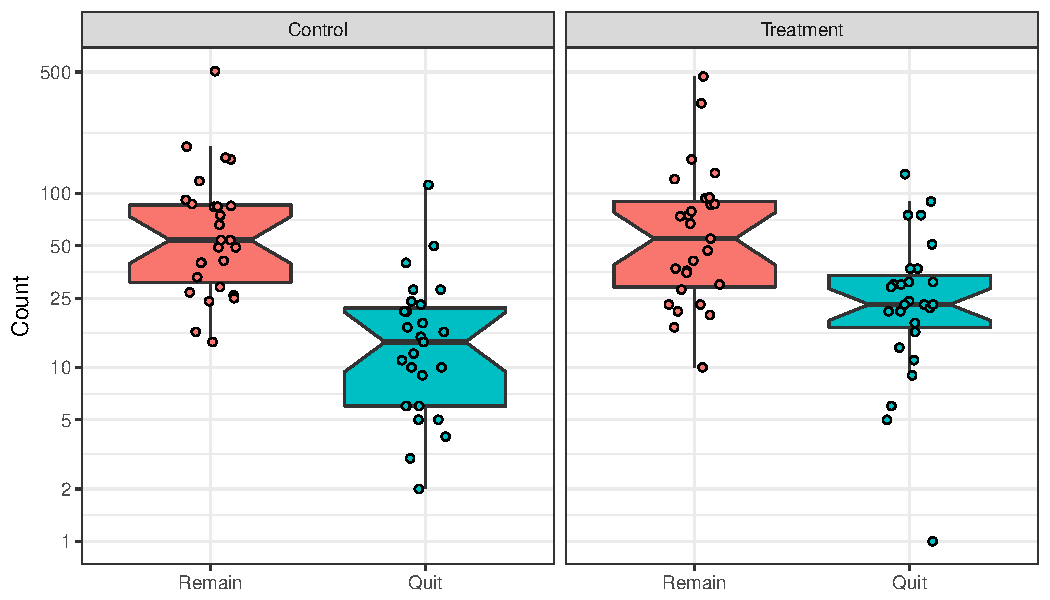
\includegraphics[width=\maxwidth]{figure/05-plot_data_smoke-1} 

}

\caption[Comparative box-plots of the distribution of patients who successfully quit smoking and those who remained smokers, in the two treatment groups]{Comparative box-plots of the distribution of patients who successfully quit smoking and those who remained smokers, in the two treatment groups. It is evident that there are more successful patients quitting smoking in the treatment group than in the control group. The raw odds ratio of quitting smoking (treatment vs. control) is 1.66.}\label{fig:plot.data.smoke}
\end{figure}


\end{knitrout}
A summary of the data is displayed by the box-plot in \cref{fig:plot.data.smoke}.
On the whole, there are a total of 5,908
% study.size[length(study.size)]
patients, and they are distributed roughly equally among the control and treatment groups (46.3\% and 53.7\% respectively, on average).
From the box-plots, it is evident that there are more patients who quit smoking in the treatment group as compared to the placebo control group.
There are various measures of treatment effect size, such as risk ratio or risk differences, but we shall concentrate on \emph{odds ratios} as defined by \index{odds}\index{odds!ratio}
\[
  \text{odds ratio} = \frac{\text{odds of quitting smoking in \emph{treatment} group}}
  {\text{odds of quitting smoking in \emph{control} group}}.
\]
The odds of quitting smoking in either group is defined as
\[
  \text{odds} = \frac{\Prob(\text{quit smoking})}{1 - \Prob(\text{quit smoking})},
\]
and these probabilities, odds and ultimately odds ratio can be estimated from sample proportions.
This raw odds ratio for all study groups is calculated as $1.66 = e^{0.50}$.
It is also common for the odds ratio to be reported on the log scale (usually as a remnant of logistic models).
A value greater than one for the odds ratio (or equivalently, greater than zero for the log odds ratio) indicates a significant treatment effect.

A random-effects analysis using a multilevel logistic model has been considered by \citet{agresti2000tutorial}.
Let $i=1,\dots,n_k$ index the patients in study group $k \in \{1,\dots,27\}$.
For patient $i$ in study $j$, $p_{ik}$ denotes the probability that the patient has successfully quit smoking.
Additionally, $x_{ik}$ is the centred dummy variable indicating patient $i$'s treatment group in study $k$.
These take on two values: 0.5 for treated patients and -0.5 for control patients.
The logistic random-effects model is
\begin{gather*}
  \log \left( \frac{p_{ij}}{1-p_{ij}} \right) = \beta_{0j} + \beta_{1j}x_{ij} \\
  \intertext{with}
  \begin{pmatrix} \beta_{0j} \\ \beta_{1j} \end{pmatrix}
  \sim \N \left(
  \begin{pmatrix} \beta_0 \\ \beta_1 \end{pmatrix},
  \begin{pmatrix} \sigma_0^2 & \sigma_{01} \\ \sigma_{01} & \sigma_1^2 \\ \end{pmatrix}
  \right)
\end{gather*}
\citet{agresti2000tutorial} also made the additional assumption $\sigma_{01} = 0$, so that, coupled with the contrast coding used for $x_{ik}$, the total variance $\Var(\beta_{0k} + \beta_{1j}x_{ik})$ would be constant in both treatment groups.
The overall log odds ratio is represented by $\beta_1$, and this is estimated as $0.57 \approx \log 1.76$.

In an I-prior model, the Bernoulli probabilities $p_{ik}$ are regressed against the treatment group indicators $x_{ik}$ and also the patients' study group $k$ via the regression function $f$ and a probit link:
\begin{align*}
  \Phi^{-1}(p_{ik})
  &= f(x_{ik}, k) \\
  &= f_1(x_{ik}) + f_2(k) + f_{12}(x_{ik}, j).
\end{align*}
We have decomposed our function $f$ into three parts: $f_1$ represents the treatment effect, $f_2$ represents the effect of the study groups, and $f_{12}$ represents the interaction effect between the treatment and study group on the modelled probabilities.
As both $x_{ik}$ and $k$ are nominal variables, the functions $f_1$ and $f_2$ both lie in the Pearson RKHS of functions $\cF_1$ and $\cF_2$, each with RKHS scale parameters $\lambda_1$ and $\lambda_2$.
As such, it does not matter how the $x_{ik}$ variables are coded (dummy coding 0, 1 vs. centred coding -0.5, 0.5) as the scaling of the function is determined by the RKHS scale parameters.
The interaction effect $f_{12}$ lies in the RKHS tensor product $\cF_1 \otimes \cF_2$.
In the I-probit model, there are only two parameters to estimate, while in the standard logistic random-effects model, there are six.
The results of the I-prior fit are summarised in the table below.


\newcolumntype{R}[1]{>{\raggedleft\arraybackslash}p{#1}}
\begin{table}[hbt]
  \centering
  \caption{Results of the I-probit model fit for three models.}
  \label{tab:mod.compare.smoke}
  \begin{tabular}{lrrrR{2cm}}
  \toprule
  Model & ELBO & Error rate (\%) & Brier score & No. of parameters \\
  \midrule
  $f_1$
  &-3210.76
  &23.65
  &0.179 & 1 \\
  $f_1+f_2$
  &-3142.24
  &29.30
  &0.206 & 2 \\
  $f_1+f_2+f_{12}$
  &-3091.20
  &23.48
  &0.168 & 2 \\
  \bottomrule
  \end{tabular}
\end{table}

The approximated marginal log-likelihood value for the I-prior model (i.e. variational lower bound), the Brier score for each model and the number of RKHS scale parameters estimated in the model are reported in \cref{tab:mod.compare.smoke}. Three models were fitted:
1) a model with only the treatment effect;
2) a model with a treatment effect and a study group effect; and
3) Model 2 with the additional assumption that treatment effect varies across study groups.
Model 1 disregards the study group effects, while Model 2 assumes that the effectiveness of the nicotine gum treatment does not vary across study groups (akin to a varying-intercept model).
A model comparison using the evidence lower bound indicates that Model 3 has the highest value, and the difference is significant from a Bayes factor standpoint---$\BF(M_3,M_1)$ and $\BF(M_3,M_2)$ are both greater than 150.
% with both Bayes factor comparing Model 3 against Models 1 and 2 being greater than 150.
% $\BF(M_3, M_1)iprior::dec_plac(exp(l[3] - l[1]), 2)$ and $\BF(M_3, M_2)iprior::dec_plac(exp(l[3] - l[2]), 2)$.
% Although not soundly based in theory, we may compare variational lower bounds of the three models for model selection as a proxy to using the true log-likelihood value.
% In this case, Model 3 has the highest lower bound value.
The misclassification rate and Brier score indicates good predictive performance of the models, and there is not much to distinguish between the three although Model 3 is the best out of the three models.

\begin{knitrout}
\definecolor{shadecolor}{rgb}{1, 1, 1}\color{fgcolor}\begin{figure}[p]

{\centering 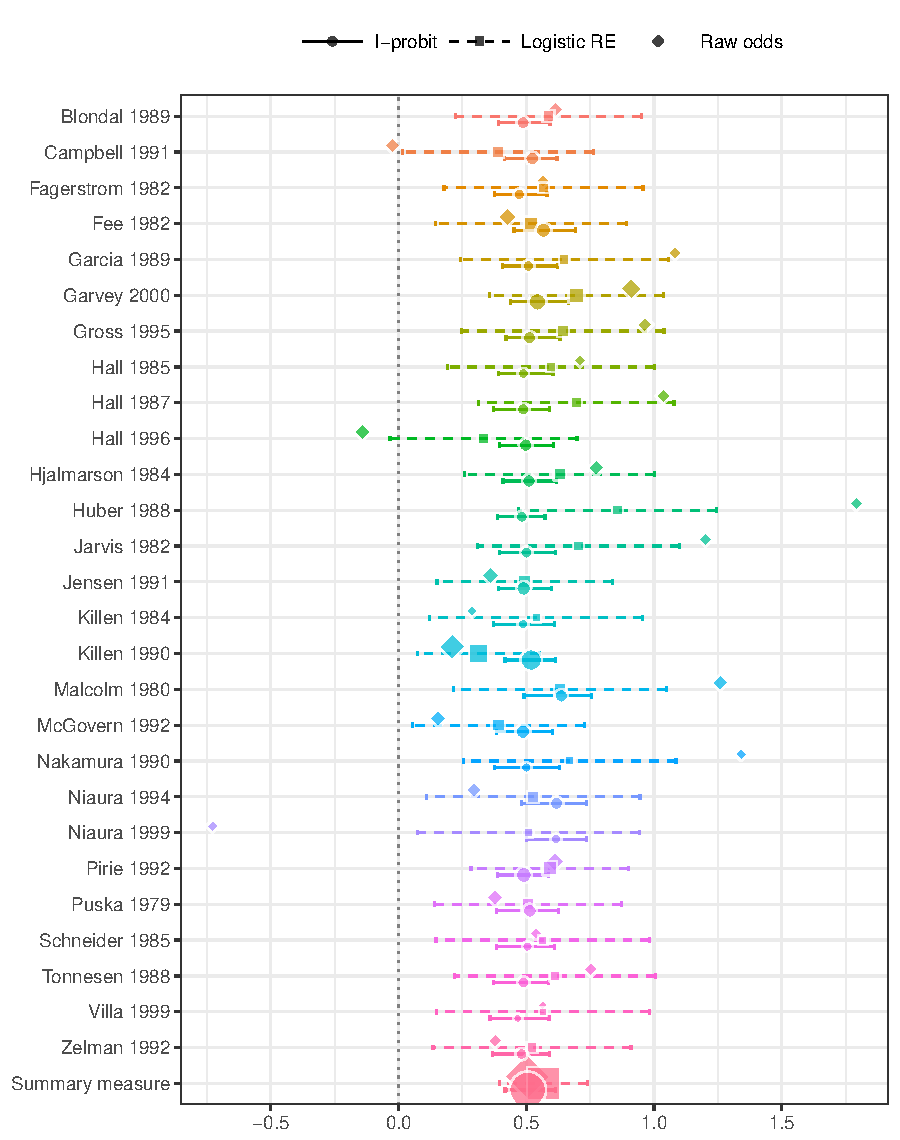
\includegraphics[width=\linewidth]{figure/05-smoke_forest_plot-1} 

}

\caption[Forest plot of effect sizes (log odds ratios) in each group as well as the overall effect size together with their 95\% confidence bands]{Forest plot of effect sizes (log odds ratios) in each group as well as the overall effect size together with their 95\% confidence bands. The plot compares the raw log odds ratios, the logistic random-effect estimates, and the I-prior estimates. Sizes of the points indicate the relative sample sizes per study group.}\label{fig:smoke.forest.plot}
\end{figure}


\end{knitrout}

Unlike in the logistic random-effects model, where the log odds ratio can be read off directly from the coefficients, with an I-prior probit model the log odds ratio needs to be calculated manually from the fitted probabilities. \index{log odds ratio}\index{log odds ratio|seealso{odds ratio}}
The probabilities of interest are the probabilities of quitting smoking under each treatment group for each study group $k$---call these $p_k(\text{treatment})$ and $p_k(\text{control})$.
That is,
\begin{align*}
  p_k(\text{treatment}) &= \Phi\big( \hat\nu(\text{treatment}, k) \big) \\
  p_k(\text{control})   &= \Phi\big( \hat\nu(\text{control}, k) \big),
\end{align*}
where $\hat \nu$ represents the standardised posterior mean estimate for the regression functions which are distributed according to
\[
  f(x_{ik},k)|\by,\hat\theta \sim \N\big(\hat\mu(x_{ik}, k), \hat\sigma^2(x_{ij}, k) \big),
\]
with $x_{ik}\in\{\text{treatment}, \text{control} \}$ and $k \in \{1,\dots,27\}$  (see details in \cref{sec:iprobitpostest}).
The log odds ratio for each study group can then be calculated as usual.
For the overall log odds ratio, the probabilities that are used are the averaged probabilities weighted according to the sample sizes in each group.
This has been calculated as $0.51 \approx \log 1.66$, slightly lower than both the raw log odds ratio and the log odds ratio estimated by the logistic random-effects model.
This can perhaps be attributed to some shrinkage of the estimated probabilities due to placing a prior with zero mean on the regression functions.

The credibility intervals for the log odds ratios in the forest plot of \cref{fig:smoke.forest.plot} are also noticeably narrower under an I-prior compared to the fitted multilevel model.
One explanation is that empirical Bayes estimates, such as the I-probit estimates under a variational EM framework, tend to underestimate the variability in the estimates because the variability in the parameters are ignored when point estimates are used, compared to distributions in a true Bayesian estimation framework.

\subsection{Multiclass classification: Vowel recognition data set}
\index{classification!multiclass}
\index{Deterding data set|see{vowel recognition data set}}
\index{vowel recognition data set}
\index{canonical kernel/RKHS}
\index{fBm kernel/RKHS}
\index{SE kernel/RKHS}





We illustrate multiclass classification using I-priors on a speech recognition data set\footnotemark~with $m = 11$ classes to be predicted from digitized low pass filtered signals generated from voice recordings.
Each class corresponds to a vowel sound made when pronouncing a specific word.
The words that make up the vowel sounds are shown in \cref{tab:vowel}. Each word was uttered once by multiple speakers, and the data are split into a training and a test set.
Four males and four female speakers contributed to the training set, while four male and three female speakers contributed to the test set.
The recordings were manipulated using speech processing techniques, such that each speaker yielded six frames of speech from the eleven vowels, each with a corresponding 10-dimensional numerical input vector (the predictors).
This means that the size of the training set is $8 \times 6 \times 11 = 528$, while $7 \times 6 \times 11 = 462$ data points are available for testing the predictive performance of the models.
This data set is also known as Deterding's vowel recognition data (after the original collector, \cite{deterding1989speaker}).
Machine learning methods such as neural networks and nearest neighbour methods were analysed by \citet{robinson1989dynamic}.

\footnotetext{Data is publicaly available from the UCI Machine Learning Repository, URL: \url{https://archive.ics.uci.edu/ml/datasets/Connectionist+Bench+(Vowel+Recognition+-+Deterding+Data)}.}

\begin{table}[htb]
\centering
\caption{The eleven words that make up the classes of vowels.}
\label{tab:vowel}
\begin{tabular}{llllllllll}
\toprule
Class & Label          & Vowel & Word &  && Class & Label          & Vowel & Word  \\
\midrule
1     & \texttt{hid} & \dsil{iː}    & heed &&  & 7     & \texttt{hOd} & \dsil{ɒ}    & hod   \\
2     & \texttt{hId} & \dsil{ɪ}     & hid  &&  & 8     & \texttt{hod} & \dsil{ɔː}   & hoard \\
3     & \texttt{hEd} & \dsil{ɛ}     & head &&  & 9     & \texttt{hUd} & \dsil{ʊ}    & hood  \\
4     & \texttt{hAd} & \dsil{a}     & had  &&  & 10    & \texttt{hud} & \dsil{uː}   & who'd \\
5     & \texttt{hYd} & \dsil{ʌ}     & hud  &&  & 11    & \texttt{hed} & \dsil{əː}   & heard \\
6     & \texttt{had} & \dsil{ɑː}    & hard &&  &       &              &             &       \\
\bottomrule
\end{tabular}
\end{table}

We will fit the data using an I-probit model with the canonical linear kernel, fBm-0.5 kernel, and the SE kernel with lengthscale $l=1$.
% We assume $m = 11$ distinct I-priors corresponding to the latent variables in each class, thus there are 11 unique intercepts and 11 RKHS scale parameters to estimate in each model.
Each model took roughly 13 seconds per iteration in fitting the training data set ($n=528$).
In particular, the canonical kernel model took a long time to converge, with each variational inference iteration improving the lower bound only slighly each time.
In contrast, both the fBm-0.5 and SE model were quicker to converge.
Multiple restarts from different random seeds were conducted, and we found that they all converged to a similar lower bound value.
This alleviates any concerns that the model might have converged to different multiple local optima.

\begin{knitrout}
\definecolor{shadecolor}{rgb}{1, 1, 1}\color{fgcolor}\begin{figure}[htb]

{\centering \subfloat[Canonical kernel\label{fig:vowel.confusion.matrix1}]{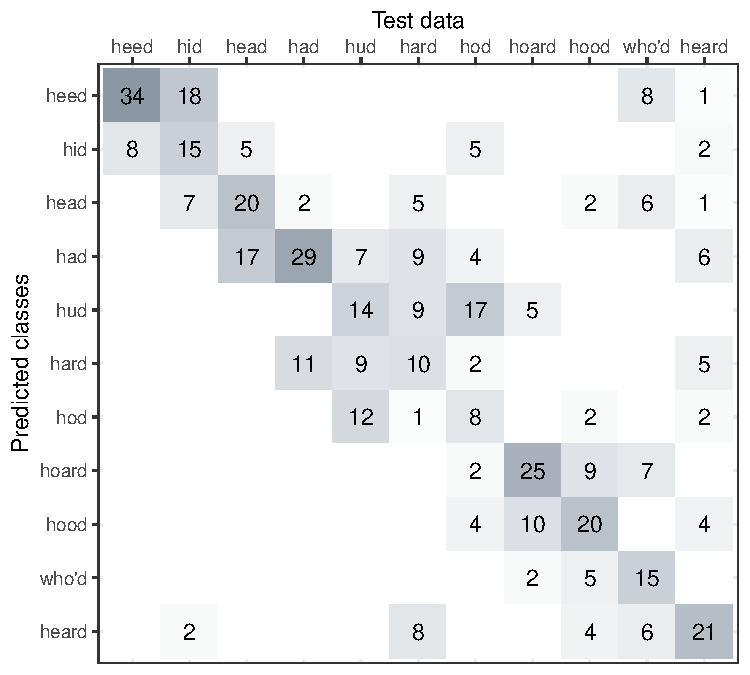
\includegraphics[width=0.485\linewidth]{figure/05-vowel_confusion_matrix-1} }
\subfloat[fBm-0.5 kernel\label{fig:vowel.confusion.matrix2}]{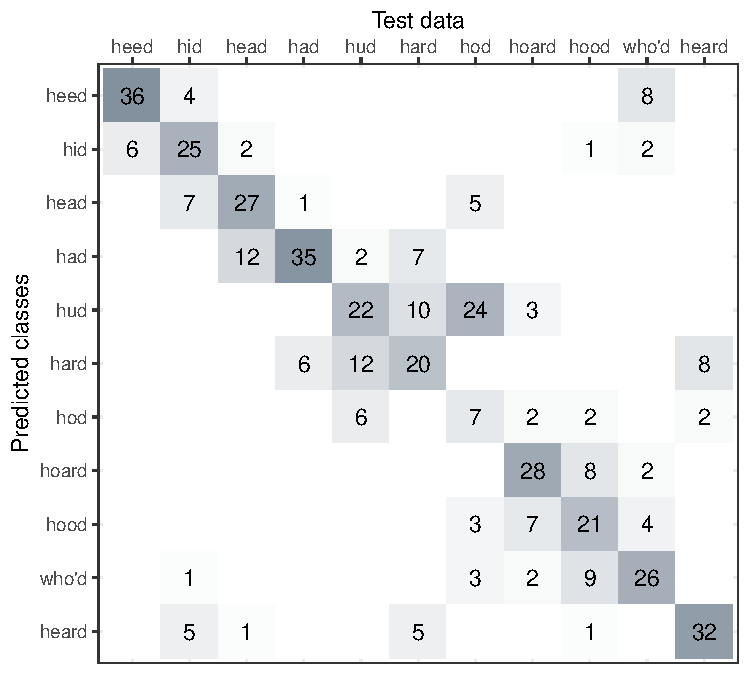
\includegraphics[width=0.485\linewidth]{figure/05-vowel_confusion_matrix-2} }
\subfloat[SE kernel\label{fig:vowel.confusion.matrix3}]{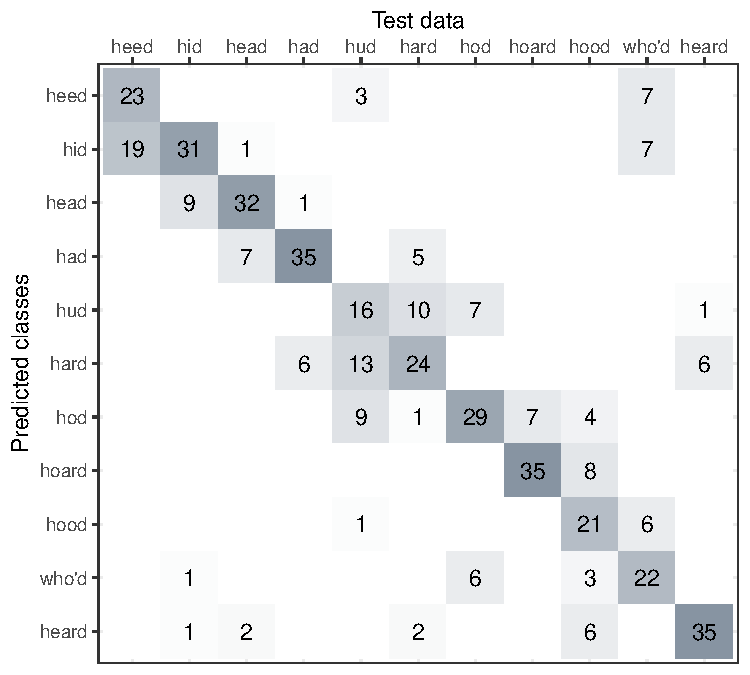
\includegraphics[width=0.485\linewidth]{figure/05-vowel_confusion_matrix-3} }

}

\caption[Confusion matrices for the vowel classification problem in which predicted values were obtained from the I-probit models]{Confusion matrices for the vowel classification problem in which predicted values were obtained from the I-probit models. The maximum value for any cell is 42 (seven speakers delivered six frames of speech per vowel). Blank cells indicate nil values.}\label{fig:vowel.confusion.matrix}
\end{figure}


\end{knitrout}

A good way to visualise the performance of model predictions is through a confusion matrix, as shown in \cref{fig:vowel.confusion.matrix}.
The numbers in each row indicate the instances of a predicted class, while the numbers in the column indicate instances of the actual classes, while nil values are indicated by blank cells.
% A quick glance of the plots seem to favour the fBm-0.5 kernel as having better predictions.
% There are a lot more misclassifications when using the canonical kernel.
% Under the fBm-0.5 model, the model makes understandable mistakes - confusing very similar words, especially `hod' and `hud'.

Comparisons to other methods that had been used to analyse this data set is given in \cref{tab:vowel.tab}.
In particular, the I-probit model is compared against 1) linear regression; 2) logistic linear regression; 3) linear and quadratic discriminant analysis; 4) decision trees; 5) neural networks; 6) $k$-nearest neighbours; and 7) flexible discriminant analysis.
All of these methods are described in further detail in \citet[chs. 4 \& 12, table 12.3]{friedman2001elements}.
The I-probit model using both the fBm-0.5 and SE kernel offers one of the best out-of-sample classification error rates (34.4\%) of all the methods compared.
The linear I-probit model is seen to be comparable to logistic regression, linear and quadratic discrimant analysis, and also decision trees.
It also provides significant improvement over multiple linear regression.

\begin{table}
  \caption{Results of various classification methods for the vowel data set.}
  \label{tab:vowel.tab}
  \centering
  \begin{tabular}{l r r}
  \toprule
  \Bot &\multicolumn{2}{c}{Error rate (\%)} \\
  \cline{2-3}
  \Top Model & Train & Test \\
  \midrule
  \emph{I-probit} \\
  \hspace{0.5em} Linear
  & 29
  & 54 \\
  \hspace{0.5em} Smooth (fBm-0.5)
  & 22
  & 40 \\
  \hspace{0.5em} Smooth (SE-1.0)
  & 7
  & 34 \\
  \\
  \emph{Others} \\
  \hspace{0.5em} Linear regression               & 48 & 67 \\
  \hspace{0.5em} Logistic regression             & 22 & 51
  \\[0.5em]
  \hspace{0.5em} Linear discriminant analysis    & 32 & 56 \\
  \hspace{0.5em} Quadratic discriminant analysis & 1  & 53
  \\[0.5em]
  \hspace{0.5em} Decision trees                  & 5  & 54 \\
  \hspace{0.5em} Neural networks                 &    & 45 \\
  \hspace{0.5em} $k$-nearest neighbours          &    & 44
  \\[0.5em]
  \hspace{0.5em} FDA/BRUTO                       & 6  & 44 \\
  \hspace{0.5em} FDA/MARS                        & 13 & 39 \\
  \bottomrule
  \end{tabular}
\end{table}

\subsection{Spatio-temporal modelling of bovine tuberculosis in Cornwall}
\index{spatio-temporal model}
\index{BTB data set}
\index{ANOVA!kernel/RKKS}
\index{fBm kernel/RKHS}
\index{Pearson kernel/RKHS}



Data containing the number of breakdows of bovine tubercolosis (BTB) in Cornwall, the locations of the infected animals, and the year of occurence is analysed.
The interest, as motivated by veterinary epidimiology, is to understand whether or not there is spatial segregation of the infection of the herds, and whether there is a time-element to the presence or absence of this spatial segregation.
There has been previous work done to analyse this data set.
\citet{diggle2005nonparametric} developed a non-parametric method to estimate spatial segregation using a multivariate point process.
The occurrences are modelled as Poisson point processes, and spatial segregation is said to have occured if the model-estimated type-specific breakdown probabilities at any given location are not significantly different from the sample proportions.
The authors estimated the probabilities via kernel regression, and the test statistic of interest had to be estimated via Monte Carlo methods.
Other works include \citet{diggle2013spatial}, who used a fully Bayesian approach for spatio-temporal multivariate log-Gaussian Cox processes, which is implemented in the \proglang{R} package \pkg{lgcp} \citep{taylor2013lgcp}.

\begin{knitrout}
\definecolor{shadecolor}{rgb}{1, 1, 1}\color{fgcolor}\begin{figure}[htb]

{\centering 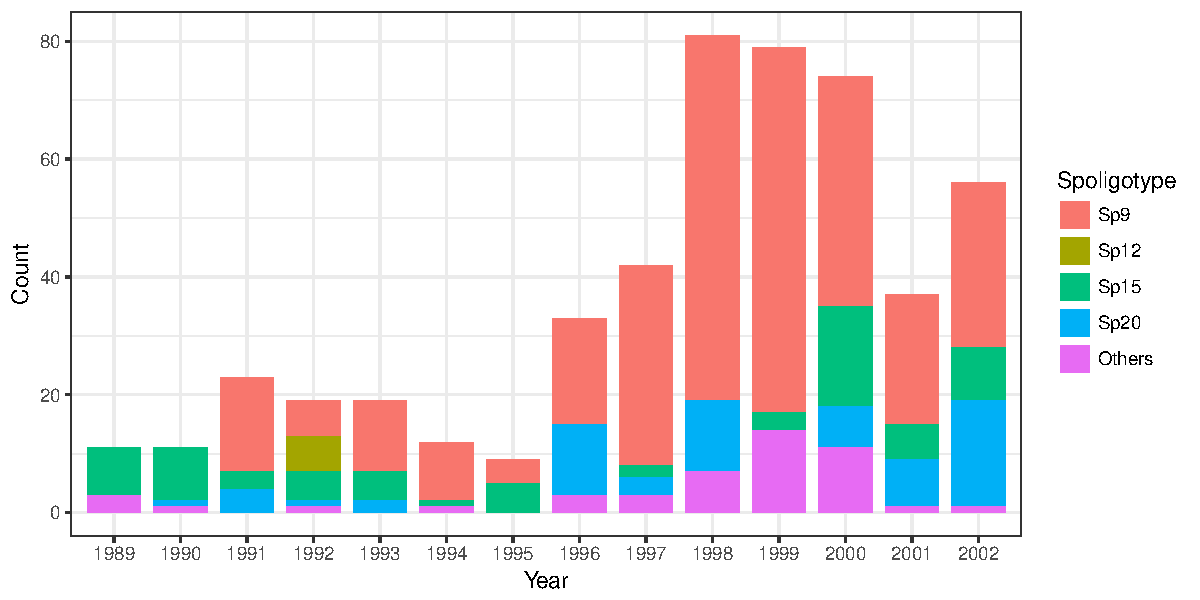
\includegraphics[width=\linewidth]{figure/05-plot_cow-1} 

}

\caption[Distribution of the different types (Spoligotypes) of bovine tubercolosis affecting herds in Cornwall over the period 1989 to 2002]{Distribution of the different types (Spoligotypes) of bovine tubercolosis affecting herds in Cornwall over the period 1989 to 2002.}\label{fig:plot.cow}
\end{figure}


\end{knitrout}

The data set contains $n=919$ recorded cases over a span of 14 years.
For each of the cases, spatial data pertaining to the location of the farm (Northings and Eastings, measured in kilometres) are available.
Originally, 11 unique spoligotypes were recorded in the data, with the four most common spoligotypes being Sp9 ($m=1$), Sp12 ($m=2$), Sp15 ($m=3$) and Sp20 ($m=4$), as shown by the histogram in \cref{fig:plot.cow}.
We had grouped the remaining seven spoligotypes into an `Others' category ($m=5$), so that the problem becomes a multinomial regression with five distinct outcomes.

\begin{knitrout}
\definecolor{shadecolor}{rgb}{1, 1, 1}\color{fgcolor}\begin{figure}[htb]

{\centering 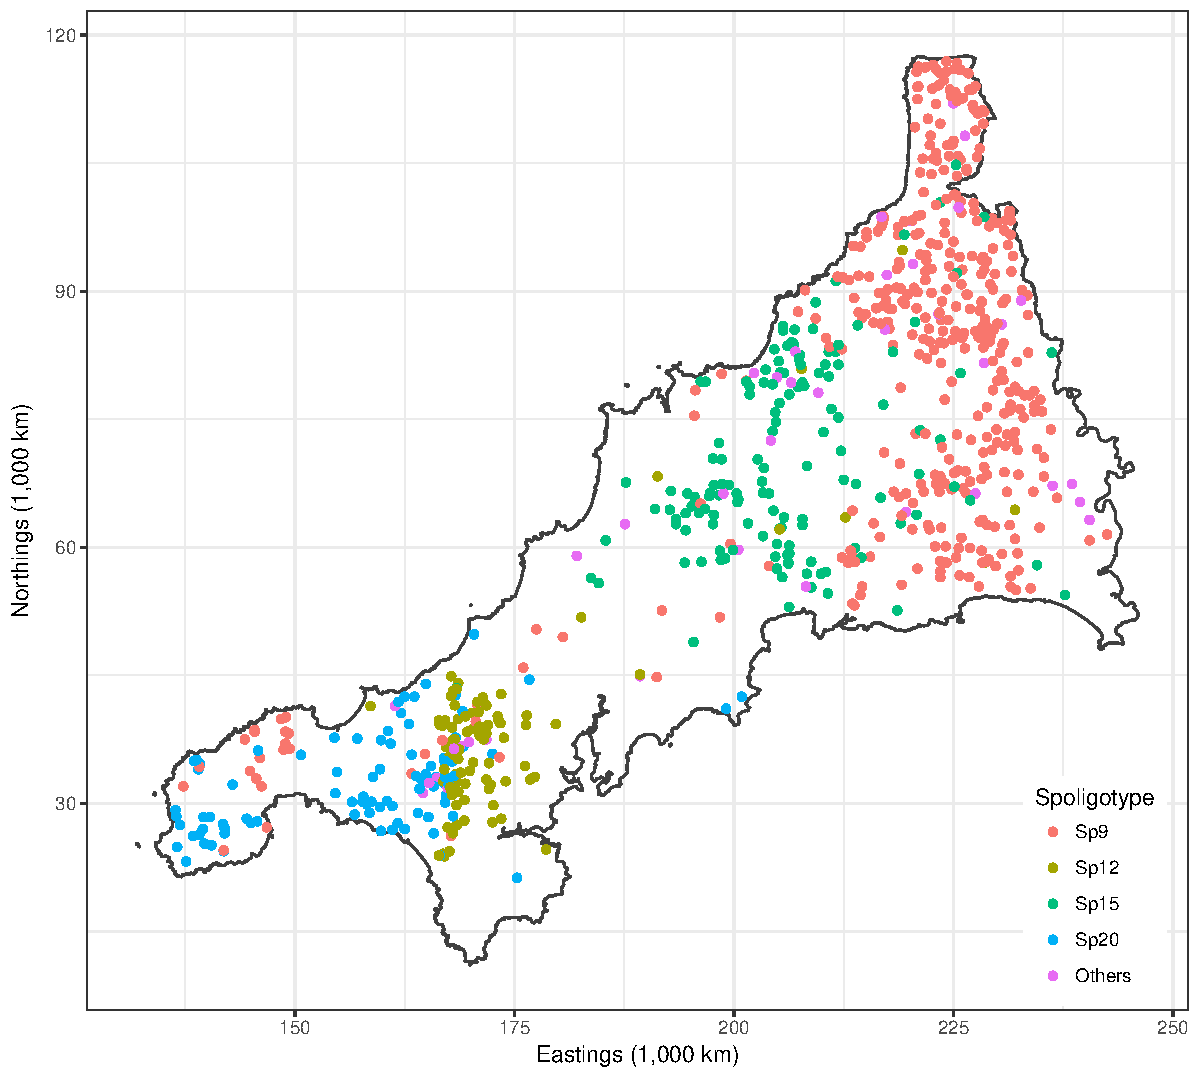
\includegraphics[width=\linewidth]{figure/05-plot_cornwall-1} 

}

\caption[Spatial distribution of all cases over the 14 years]{Spatial distribution of all cases over the 14 years.}\label{fig:plot.cornwall}
\end{figure}


\end{knitrout}

We are able to investigate any spatio-temporal patterns of infection using I-priors rather simply.
Let $p_{ij}$ denote the probability that a particular farm $i$ is infected with a BTB disease with spoligotype $j \in \{1,\dots,5\}$.
We model the transformed probabilities $g_j(p_{ij})$ as following a function which takes two covariates, i.e. the spatial data $x_1 \in \bbR^2$, and the temporal data $x_2$ (year of infection):
\begin{align*}
  p_{ij}
  &= g_j^{-1} \big( f_k(x_1, x_2) \big)_{k=1}^m \\
  &= g_j^{-1} \big( f_{1k}(x_1) + f_{2k}(x_2) + f_{12k}(x_1, x_2) \big)_{k=1}^m,
\end{align*}
where the function $g_j^{-1}:\bbR^m \to [0,1]$ is the same squashing function used in equation \cref{eq:intractablelikelihood2}.
We assume a smooth effect of space and time on the probabilities, and appropriate RKHSs for the functions $f_1 \in \cF_1$ and $f_2 \in \cF_2$ are the fBm-0.5 RKHS.
Alternatively, as per \citet{diggle2005nonparametric}, divide the data into four distinct time periods:
1) 1996 and earlier;
2) 1997 to 1998;
3) 1999 to 2000;
and finally 4) 2001 to 2002.
In this case, $x_2$ would indicate which period the infection took place in, and thus would have a nominal effect on the probabilities.
An appropriate RKHS for $f_2$ in such a case would be the Pearson RKHS.
In either case, the function $f_{12} \in \cF_1 \otimes \cF_2$ would be the ``interaction effect'', meaning that with such an effect present, the spatial distribution of the diseases are assumed to vary across the years.

\begin{sidewaystable}[p]
\caption[Results of the fitted I-probit models for the BTB contraction data set]{\label{tab:table.btb}Results of the fitted I-probit models. Estimates of the class intercepts and scale parameters, together with their respective bootstrap standard errors, are presented. For model comparison, we can look at ELBOs, error misclassification rates, and Brier scores.}
\centering
\begin{tabular}[t]{lrrrrrrrrrrr}
\toprule
\multicolumn{1}{c}{ } & \multicolumn{2}{r}{$M_0$: Intercepts only} & \multicolumn{1}{c}{ } & \multicolumn{2}{r}{$M_1$: Spatial only} & \multicolumn{1}{c}{ } & \multicolumn{2}{r}{$M_2$: Spatio-temporal} & \multicolumn{1}{c}{ } & \multicolumn{2}{r}{$M_3$: Spatio-period} \\
\cmidrule(l{2pt}r{2pt}){2-3} \cmidrule(l{2pt}r{2pt}){5-6} \cmidrule(l{2pt}r{2pt}){8-9} \cmidrule(l{2pt}r{2pt}){11-12}
  & Estimate & S.E. &   & Estimate & S.E. &   & Estimate & S.E. &   & Estimate & S.E.\\
\midrule
Intercept (Sp9) & 0.948 & 0.000 &  & 1.364 & 0.015 &  & 1.401 & 0.079 &  & 1.395 & 0.103\\
Intercept (Sp12) & -0.173 & 0.000 &  & -0.435 & 0.013 &  & -0.506 & 0.017 &  & -0.463 & 0.045\\
Intercept (Sp15) & 0.103 & 0.000 &  & -0.020 & 0.011 &  & -0.008 & 0.059 &  & -0.010 & 0.094\\
Intercept (Sp20) & -0.202 & 0.000 &  & -0.775 & 0.051 &  & -0.795 & 0.223 &  & -0.783 & 0.343\\
Intercept (Others) & -0.676 & 0.000 &  & -0.134 & 0.016 &  & -0.091 & 0.077 &  & -0.139 & 0.104\\[0.5em]
Scale (spatial) &  &  &  & 0.194 & 0.008 &  & -0.176 & 0.178 &  & 0.172 & 0.169\\
Scale (temporal) &  &  &  &  &  &  & -0.006 & 0.003 &  & -0.004 & 0.006\\
\\
ELBO & -1187.47 &  &  & -564.33 &  &  & -537.23 &  &  & -543.94 & \\
Error rate (\%) & 46.25 &  &  & 19.26 &  &  & 18.06 &  &  & 18.50 & \\
Brier score & 0.249 &  &  & 0.143 &  &  & 0.136 &  &  & 0.138 & \\
\bottomrule
\end{tabular}
\end{sidewaystable}

We fitted four different models:
\begin{itemize}
  \item \textbf{\boldmath$M_0$: Intercept only}.
  \[
    p_{ij} = g^{-1}_j\big( \alpha_k \big)_{k=1}^m
  \]
  \item \textbf{\boldmath$M_1$: Spatial segregation}.
  \[
    p_{ij} = g^{-1}_j\big(\alpha_k + f_{1k}(x_i) \big)_{k=1}^m
  \]
  $f_{1k} \in \cF_1$ Pearson RKHS.
  \item \textbf{\boldmath$M_2$: Spatio-temporal}.
  \[
    p_{ij} = g^{-1}_j\big(\alpha_k + f_{1k}(x_i) + f_{2k}(t_i) + f_{12k}(x_i,t_i) \big)_{k=1}^m
  \]
  $f_{1k} \in \cF_1$ Pearson RKHS, $f_{2k} \in \cF_2$ fBm-0.5 RKHS, and $f_{12k} \in \cF_1\otimes\cF_2$
  \item \textbf{\boldmath$M_3$: Spatio-period}.
  \[
    p_{ij} = g^{-1}_j\big(\alpha_k + f_{1k}(x_i) + f_{2k}(t_i) + f_{12k}(x_i,t_i) \big)_{k=1}^m
  \]
  $f_{1k} \in \cF_1$ Pearson RKHS, $f_{2k} \in \cF_2$ Pearson RKHS, and $f_{12k} \in \cF_1\otimes\cF_2$
\end{itemize}
Model $M_0$ corresponds to a model which ignores any spatial or temporal effects (the baseline intercept only model).
Model $M_1$ takes into account only spatial effects.
Both models $M_2$ and $M_3$ account for spatio-temporal effects, but $M_2$ assumes a smooth effect of time, while $M_3$ segregates the points into four distinct time periods for analysis.
Model comparison is easily done, and \cref{tab:table.btb} indicates that model $M_2$ has the highest ELBO of the four models, making it the preferable model.

% Alternatively, spatio-temporal effects of the BTB breakdowns can easily be inferred through the RKHS scale parameters.
% Let $h_k$, $k \in \{1,2\}$ denote the reproducing kernel of the spatial and temporal RKHSs respectively.
% Then, an I-prior on $f_j = f_{1j} + f_{2j} + f_{12j}$, $j=1,\dots,5$, takes the form
% \[
%   f_j(x_1,x_2) = \sum_{i=1}^n \big(
%   \lambda_1 h_1(x_1, x_{i1}) + \lambda_2 h_2(x_2, x_{i2}) +
%   \lambda_1\lambda_2 h_1(x_1, x_{i1}) h_2(x_2, x_{i2})
%   \big)w_{ij}
% \]
% where it is assumed $(w_{i1},\dots,w_{i5})^\top \iid \N(\bzero,\bI_5)$.
% The hypothesis of temporal significance is the same as testing the significance of the $\lambda_2$ parameter, while the test of both spatial and temporal effects are conducted on $\lambda_1$ and $\lambda_2$ simultaneously.
% From \hltodo{Chapter X}, we know that these scale parameters follow a normal posterior distribution, so we can calculate the $Z$-scores by dividing the mean by its corresponding standard deviation.
% Absolute values greater than three would satisfy a Bayesian hypothesis test of significance at the 0.01 level.
% The conclusion from \cref{tab:table.btb} is that the data supports a hypothesis for a spatio-temporal or spatio-period model.

For a more visual approach, we can look at the plots of the surface probabilities.
To obtain these probabilities, we first determined the spatial points (Northings and Eastings) which fall inside the polygon which makes up Cornwall.
We then obtained predicted probabilities for each class of disease at each location.
\cref{fig:plot.btb} was obtained using the model with spatial covariates only, thus ignoring any temporal effects.
In the case of the spatio-temporal model, we used the model which had the period formulation for time (model $M_3$).
This way, we can display the surface probabilities of the time periods in four plots only, which is more economical to exhibit within the margins of this thesis.
Note that there is no issue with using the continuous time model---we have produced an animated gif image at \url{http://phd.haziqj.ml/examples/}, showing the yearly evolution of the surface probabilities between 1989 and 2002.

\begin{knitrout}
\definecolor{shadecolor}{rgb}{1, 1, 1}\color{fgcolor}\begin{figure}[p]

{\centering 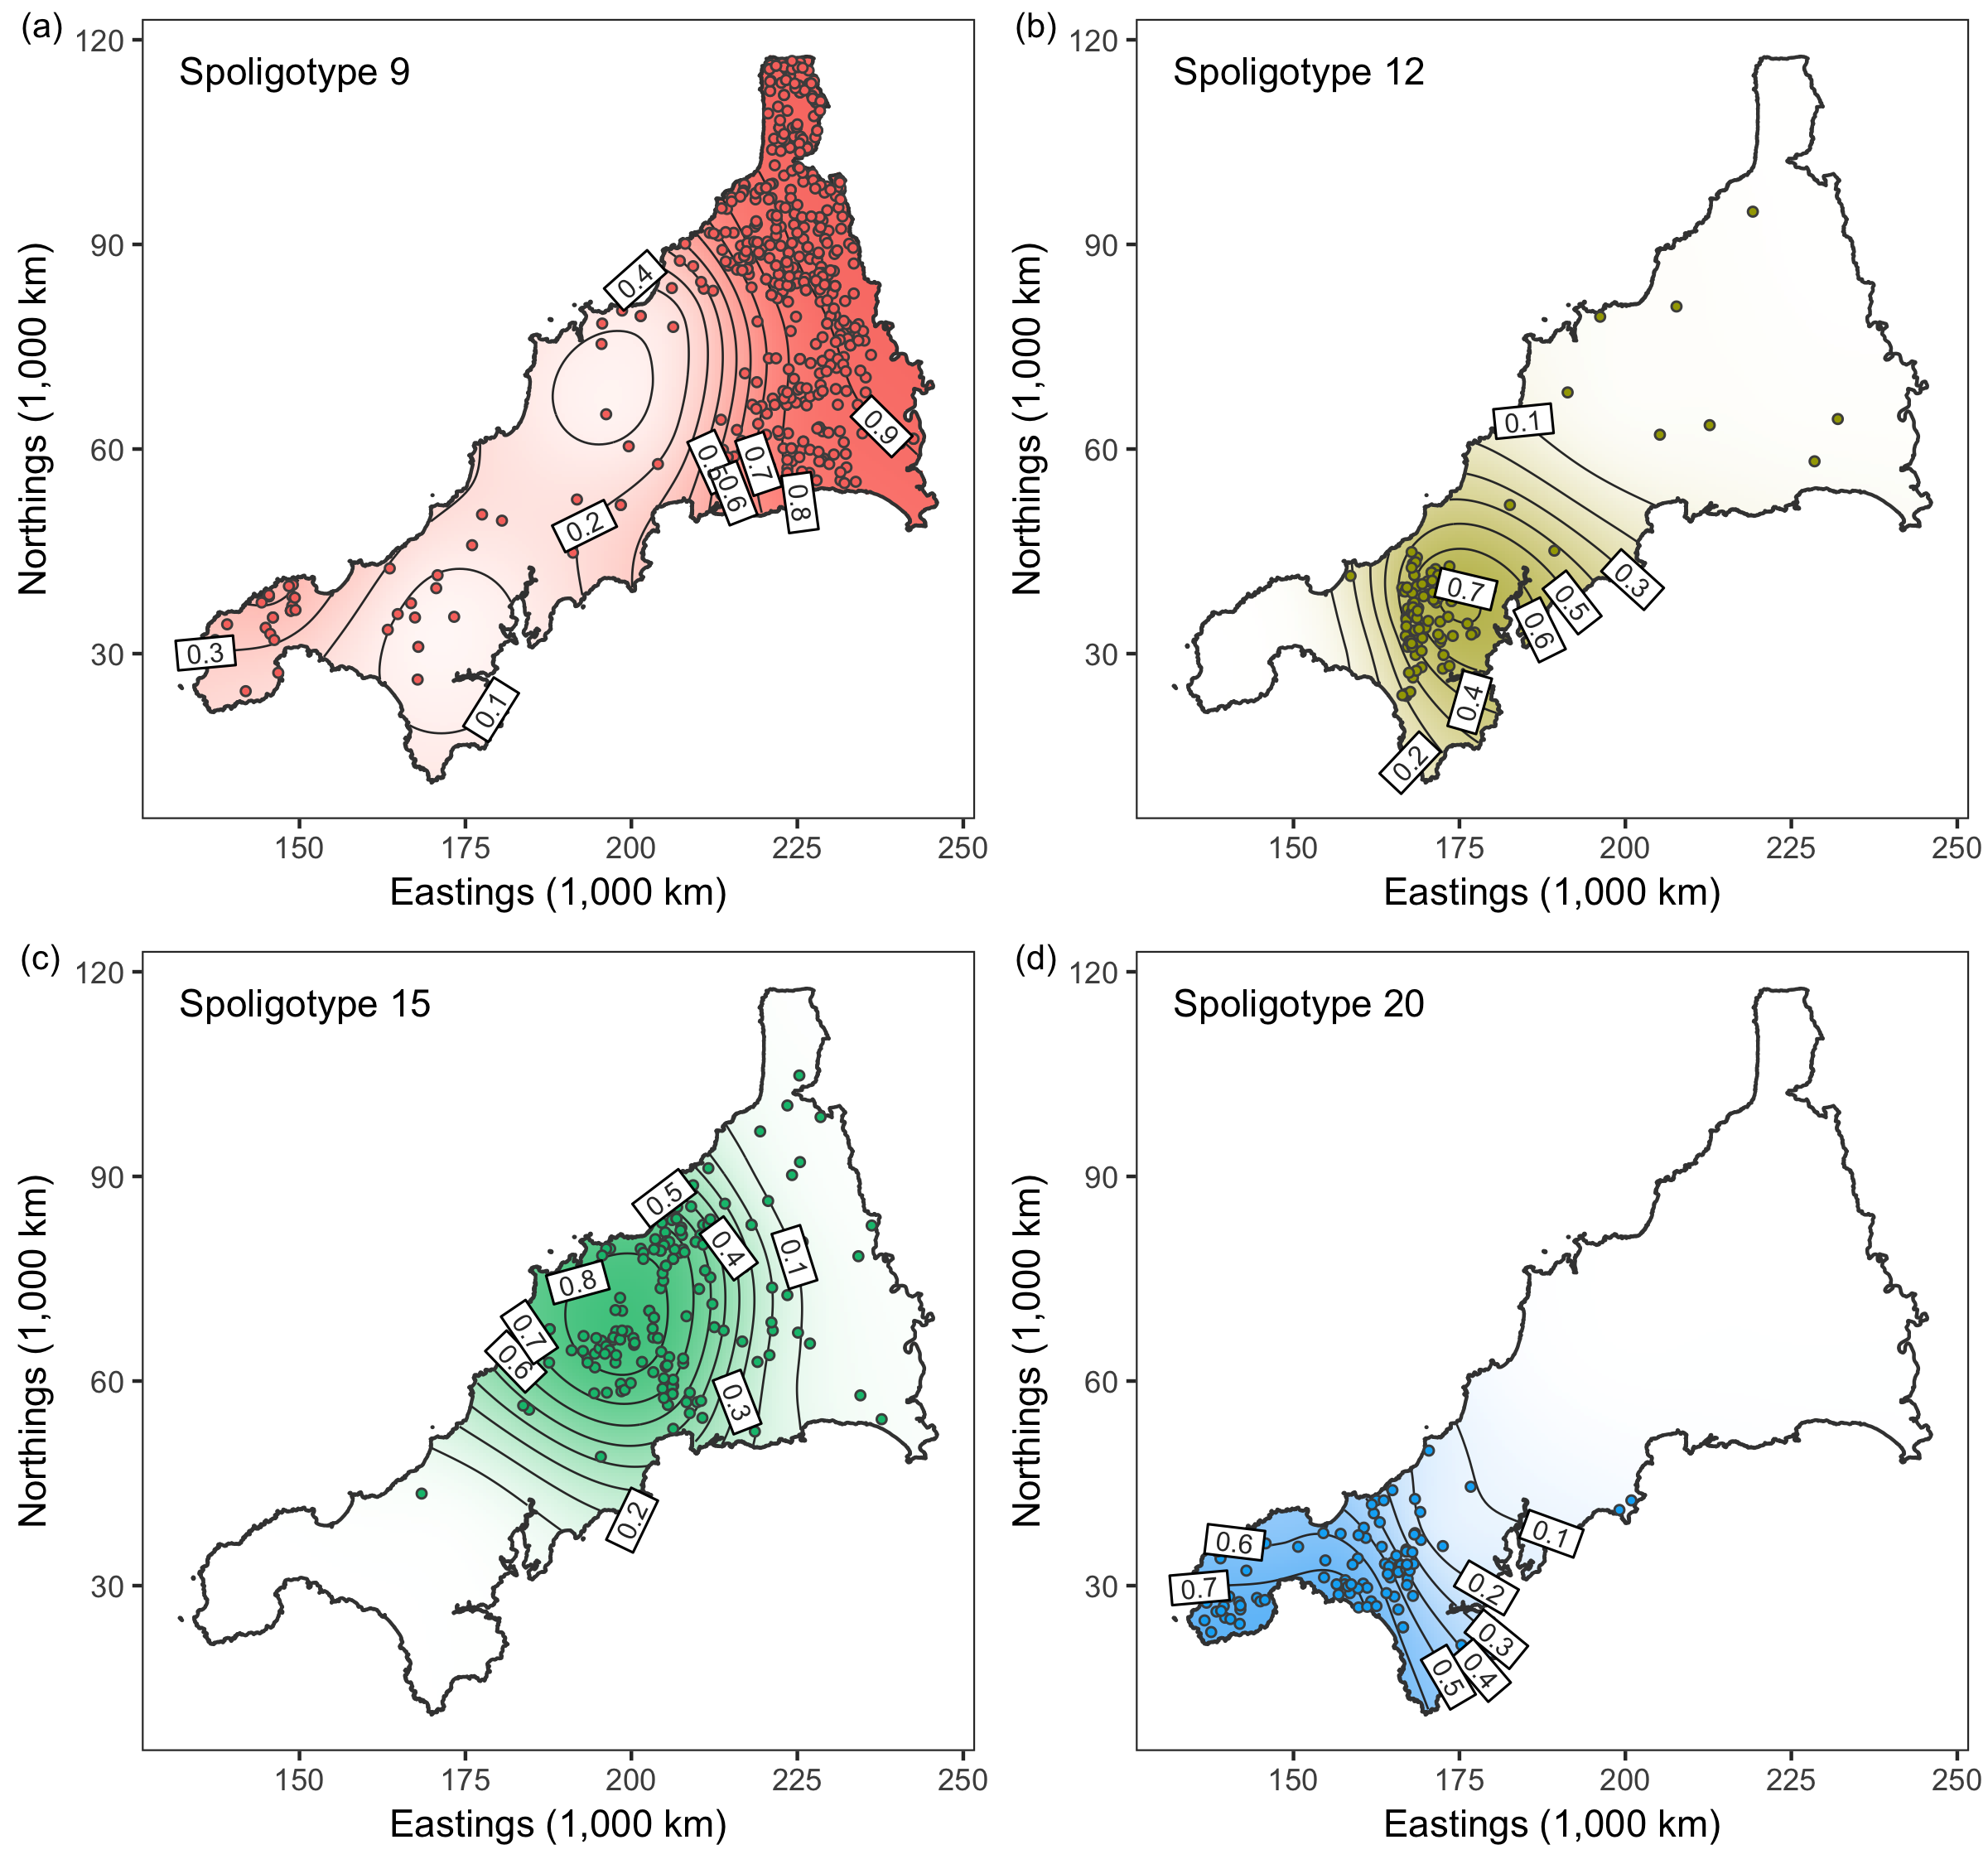
\includegraphics[width=\linewidth]{figure/05-plot_btb-1} 

}

\caption[Predicted probability surfaces of BTB contraction using model $M_1$]{Predicted probability surfaces for BTB contraction in Cornwall for the four largest spoligotypes of the bacterium \emph{Mycobacterium bovis} over the entire time period using model $M_1$.}\label{fig:plot.btb}
\end{figure}


\end{knitrout}
\begin{knitrout}
\definecolor{shadecolor}{rgb}{1, 1, 1}\color{fgcolor}\begin{figure}[p]

{\centering 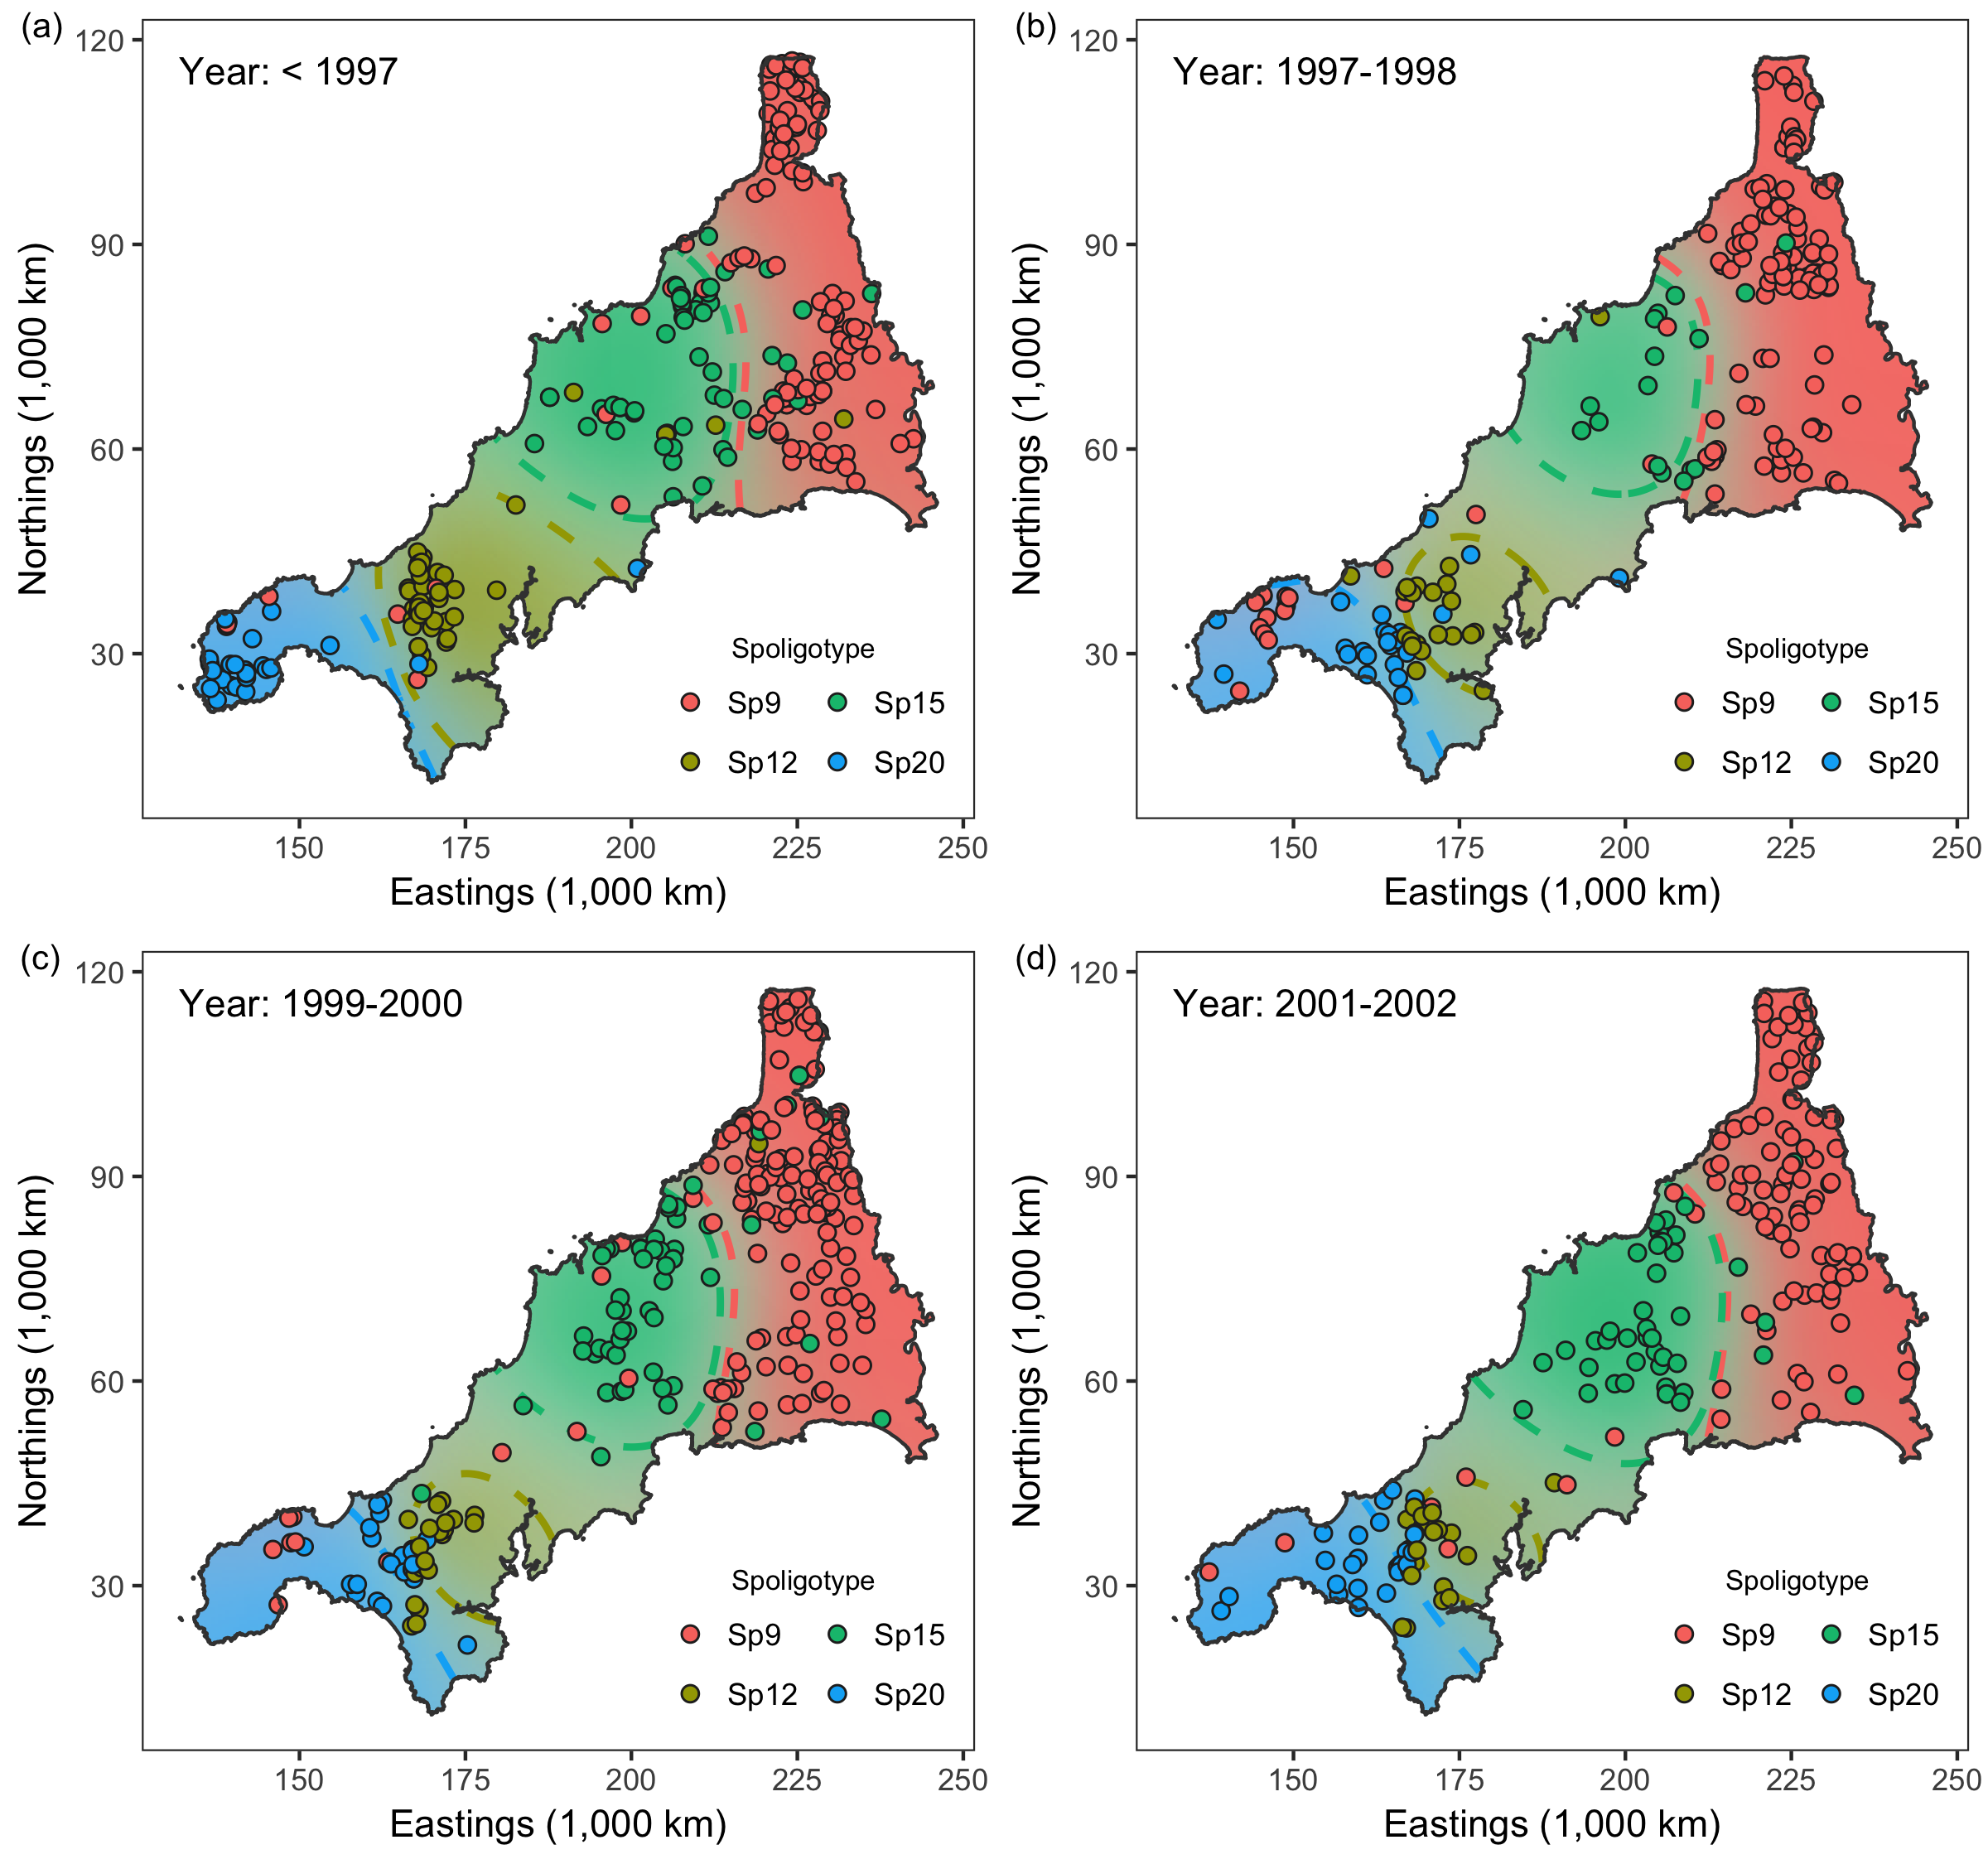
\includegraphics[width=\linewidth]{figure/05-plot_temporal_btb-1} 

}

\caption[Predicted probability surfaces of BTB contraction using model $M_3$]{Predicted probability surfaces for BTB contraction in Cornwall for the four largest spoligotypes of the bacterium \emph{Mycobacterium bovis} over four different time periods using model $M_3$.}\label{fig:plot.temporal.btb}
\end{figure}


\end{knitrout}

As the plots suggests, there is indeed spatial segregation for the four most common spoligotypes, and this is also very prominently seen from \cref{fig:plot.btb}.
In comparing the distribution of the spoligotypes over the years, we may refer to \cref{fig:plot.temporal.btb}, a series of predicted probability surface plots over the four time periods obtained from model $M_3$.
For each time period, we also superimposed the actual observations onto the predicted surface probabilities.
In addition, coloured dotted lines are displayed to indicate the ``decision boundaries'' for each of the four spoligotypes.
The most evident change is seen to the spatial distribution of spoligotype 12, with the decision boundary giving it a large area in years 1996 and earlier, but this steadily shrunk over the years.
Spoligotype 9, which is most commonly seen in the east of Cornwall, seems to have made its way down to the south-west over the years.
The other two spoligotypes seem to be rather constant over the years.

\end{document}


